\chapter{CHAIN OF RESPONSABILITY}

Pattern comportamentale avente lo scopo di evitare di associare il mittente di una richiesta al suo destinatario, dando a più di un oggetto la possibilità di gestire 
la richiesta.

Il primo oggetto della catena che riceve la richiesta, la gestisce oppure la inoltra al prossimo candidato che si comporterà nello stesso modo. 

Il client che effettuerà la richiesta, non dovrà preoccuparsi di chi dovrà gestirla, quindi è fondamentale che gli oggetti della catena abbiamo la stessa interfaccia.

\section{Applicabilità}

Quando più oggetti possono gestire una richiesta ma non è noto a priori chi lo farà oppure il caso in cui l’insieme di oggetti che possono gestire una richiesta devono 
essere specificati dinamicamente.

\section{Struttura}

\begin{figure}[h]
    \centering
    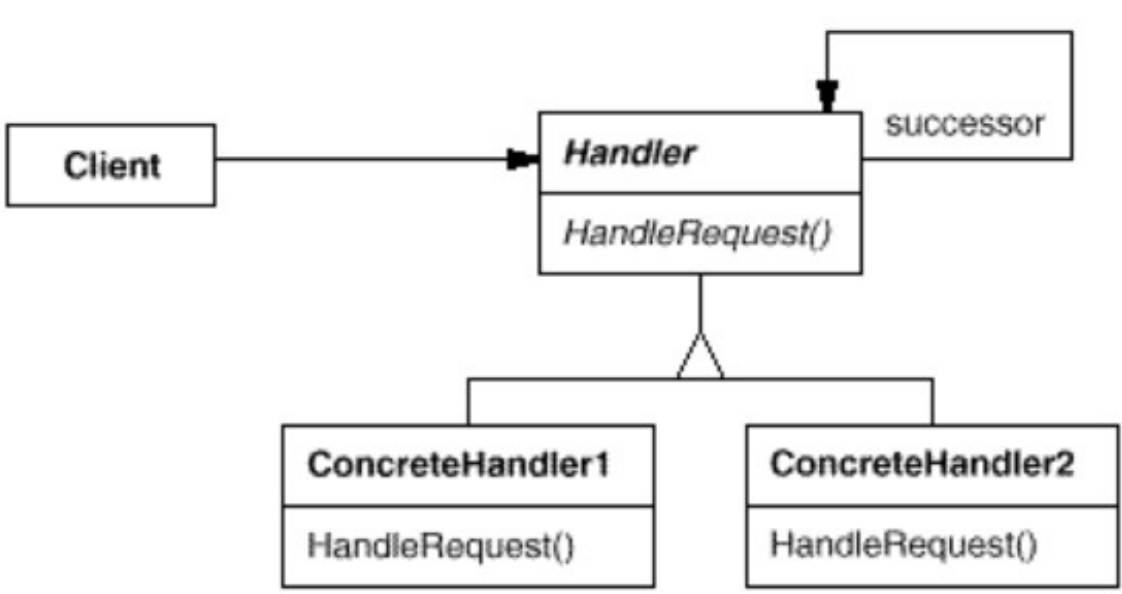
\includegraphics[width=0.4\linewidth]{../../immagini/chain_of_responsability/struttura_handler}
\end{figure}

\textbf{Handler} definisce l'interfaccia per gestire le richieste ed eventualmente implementa il riferimento al successore della catena.

\textbf{ConcreteHandler} gestisce le richieste per cui è responsabile, può accedere al successore e se può gestire la richiesta, lo fa, altrimenti la inoltra al 
successore.

\textbf{Client} invia la richiesta chiamando un metodo sul primo elemento della catena, ignorandone il tipo effettivo.

Il successore di un Handler può essere passato direttamente al costruttore oppure tramite un setter.

Nel primo caso, dopo che abbiamo creato la catena, non la possiamo più modificare, mentre nel secondo caso è consentito stando però attenti alla creazione di cicli.

\section{Conseguenze}

\textbf{Reduce coupling}, Client e ConcreteHandler sono scollegati, liberiamo il Client dal dover sapere (e non deve sapere) chi gestirà la sua richiesta. 

Un oggetto della catena non conosce la struttura della stessa ma conosce solamente il suo successore.

\textbf{Maggiore flessibilità nell'assegnazione delle responsabilità agli oggetti} dove la catena viene costruita a run-time e le responsabilità possono essere 
aggiunte o rimosse modificando la stessa.

\textbf{Ricezione non garantita}, ovvero, siccome la richiesta non ha un gestore esplicito, non c'è garanzia che venga gestita (la richiesta scorre tutta la catena).

\section{L'inoltro}

Come nel Decorator, per evitare di dimenticarsi l'inoltro, possiamo definire la logica dell'inoltro nella classe base (metodo final), chiamare al suo interno un metodo 
astratto, che conterrà la logica della gestione della richiesta che sarà poi implementata dalle sottoclassi.

\section{Decorator vs Chain of responsability}

Entrambi i pattern sembrano simili ma 

\begin{multicols}{2}
    \begin{itemize}
        \item [] ha due classi astratta;
        \item [] \textit{tutte} le classi gestiscono la richiesta;
        \item [] il componente da decorare non deve essere null;
        \item [] pattern strutturale
    \end{itemize}
\columnbreak
    \begin{itemize}
        \item [] ha una classe astratta;
        \item [] la richiesta sarà gestita da \textit{una ed una sola} classe oppure non viene gestita;
        \item [] l'ultimo componente della catena è null;
        \item [] pattern comportamentale
    \end{itemize}
\end{multicols}

\section{Lambda}

Come il Decorator, anche questo pattern simula la composizione di funzioni.

Quindi possiamo pensare di usare una lista di lambda, scorriamo questa lista che potrà terminare perchè troveremo una lambda che riesce a gestire la richiesta oppure 
perchè lista si esaurisce in quanto non abbiamo una lambda in grado di gestire la richiesta.

Però non stiamo più parlando del pattern Chain of Responsability.
